% !TEX root = main.tex
\section{Einleitung}
\label{sec:einleitung}

\subsection{Motivation}
\label{subsec:motivation}
an einleitung im paper orientieren
    • //Moderne Softwareentwicklung setzt auf Serverless- Computing, schnell skalierende Cloudarchitekturen wie Microservices (Verteilte Systeme)
    • Schnelle Start und Ausführungszeiten sind wichtig, maximaler Durchsatz zweitrangig (Kostenfrage)
    • // teilweise Installation des JRE inkl. Der Anwendung (Deployment) zu aufwendig
    • // Start-Up Zeit der JVM zu langsam
    • // HotSpotVM schon 20 Jahre alt und in C++ geschrieben (Codebasis aufwendig zu warten \& weiterzuentwickeln)
Java momentan nicht wirklich geeignet für Cloud mit schnellen kontinuierlichen Deployments und Microservices
//was ist graalvm native image und was für benefits werden geboten

\subsection{GraalVM und NativeImage}
\label{subsec:graalvmnativeimage}
Was ist GraalVM (Folie GraalVM-Architektur)
Was ist NativeImage und was ist die grundlegende Idee des Ansatzes? (Kombination von mehreren Ansätzen wie Points-To Analyse, ImageHeap, AoT Compilation)
Und welche grundlegenden Vorteile bieten Sie bzw. generell Executables

GraalVM Architektur für Native Image relevant
GraalVM nutzt als Grundlage OpenJDK
Zentrale Komponente ist der in Java geschriebene, hoch optimierende Graal-Compiler
Integriert den Graal-Compiler über das JVMCI (Java Virtual Machine Compiler Interface, JEP 243) in das OpenJDK
Dieser ersetzt den JIT(Just in Time)-Compiler C2 der HotSpot JVM (zentraler Bestandteil der JRE)
C2 ist ein aggressiv optimierender Compiler der für Serveranwendungen genutzt wird, bei denen es auf höchsten Durchsatz ankommt
Name „GraalVM“ etwas irreführend, passender wäre „OpenJDK mit Graal Compiler und zusätzlichen Werkzeugen“

NativeImage was ist das
Erlaubt es Java-Code ahead-of-time in eine eigenständige ausführbare Anwendung (executable) zu kompilieren
Das Executable läuft nicht auf der JVM sondern umfasst alle nötigen Komponenten wie Speicherverwaltung, Thread-Scheduling und Garbage Collection aus einer anderen VM -> Substrate VM
Weiterer Bestandteil des GraalVM Ökosystems
Die Substrate VM wird auch in die Executable hineinkompiliert
Closed-World Assumption erwähnen
NativeImage Vorteile

Leichte Verteilung \& Installation von Java-Programmen
Keine JRE-Installation auf den Clients notwendig
Verschiedene Jars der benötigten Bibliotheken müssen nicht mehr zusätzlich ausgeliefert werden
Wesentlich schnellere Startup Zeit durch AoT-Kompilierung
Signifikant kostengünstiger bei Serverless- und weiteren Cloudarchitekturen und häufigen Deployments (Durchsatz zweitrangig)
Performanceverhalten ist konstant und vorhersagbar
Code wird nicht mehr zur Laufzeit durch den JIT-Compiler + Profiler optimiert
Deutlich weniger Speicher, da die JVM für den JIT-Compiler nicht dauerhaft mitläuft

\newpage
\begin{figure}[h]
	\centering
	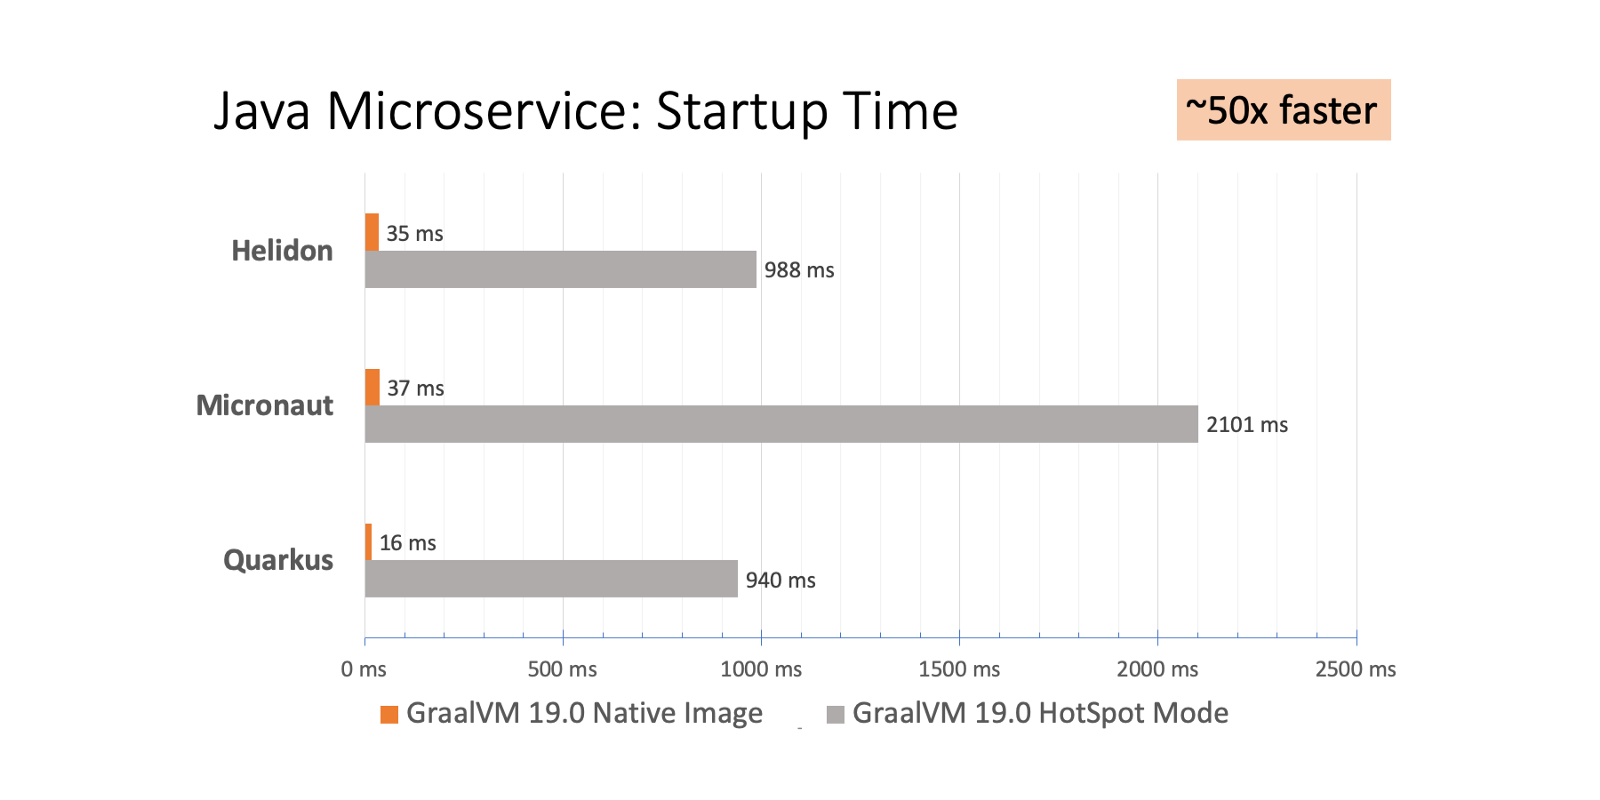
\includegraphics[width=.9\textwidth]{resources/ms_startup_time.png}
	\caption{Microservices Frameworks Startzeiten mit Native Image \parencite{GraalVMBenchmarks}}
	\label{fig:system_startuptime}
\end{figure}
\begin{figure}[h]
	\centering
	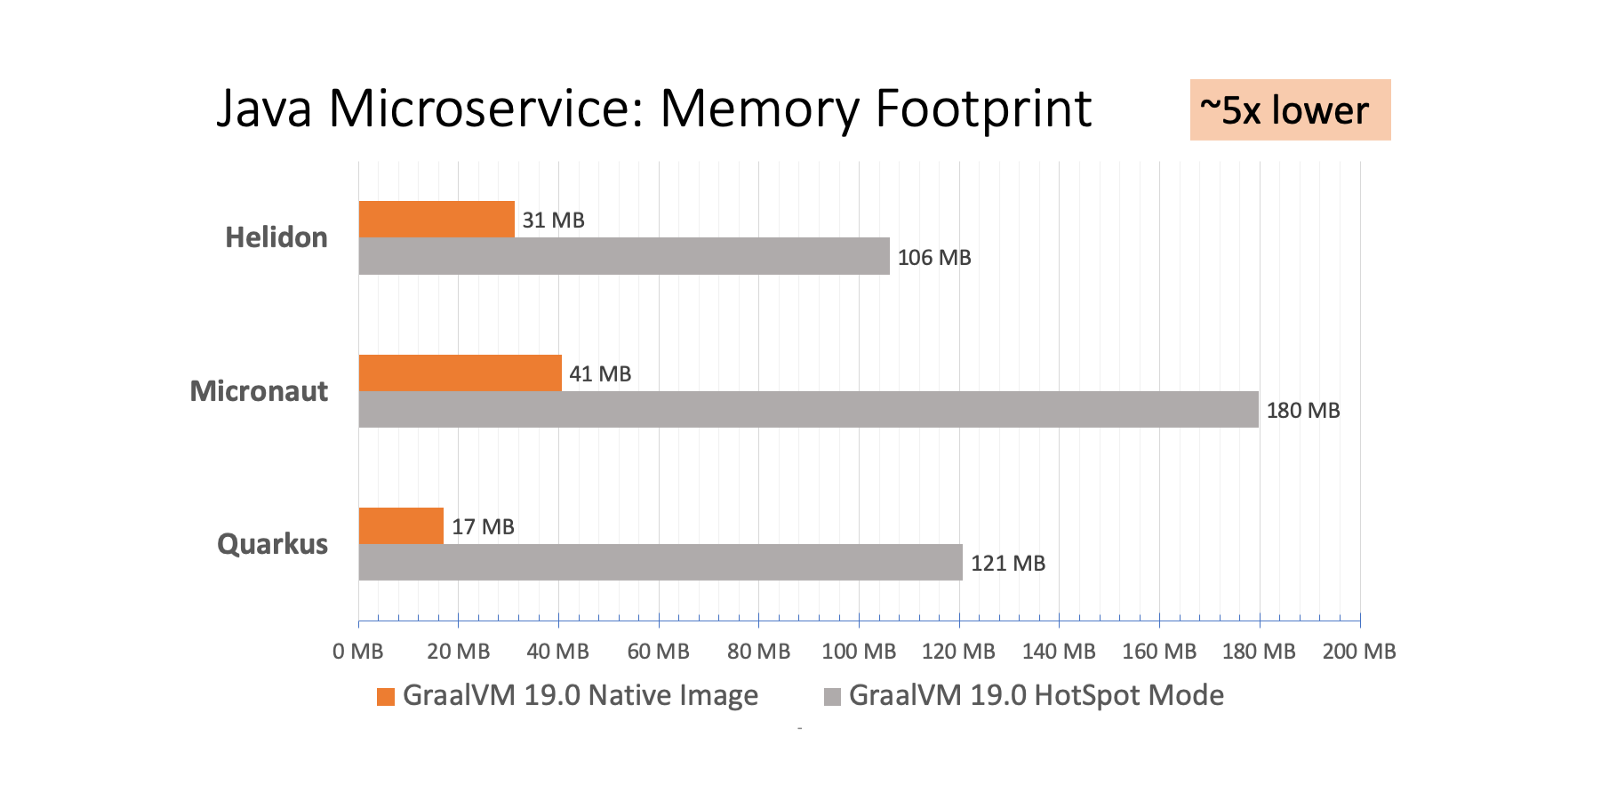
\includegraphics[width=.9\textwidth]{resources/ms_memory_footprint.png}
	\caption{Microservices Frameworks Speicherbedarf mit Native Image \parencite{GraalVMBenchmarks}}
	\label{fig:system_memory_footprint}
\end{figure}


